\documentclass{llncs}
\usepackage{graphicx}
\usepackage{url}
\usepackage[spanish]{babel}
%\usepackage[backend=biber]{biblatex} 
%\usepackage[backend=biber, style=plain, sorting=none]{biblatex}
\usepackage[spanish]{babel} \usepackage[backend=biber, sorting=none]{biblatex} \bibliography{referencias}

\begin{document}

\title{Un Sistema de Recomendación Híbrido para Mejorar Resultados}
\author{Massiel Paz Otaño \and Marlon Díaz Pérez \and Albaro Suárez Valdes}
\authorrunning{M. Paz, M. Díaz, A. Suárez}
\institute{Facultad de Matemáticas y Ciencias de la Computación, La Habana, Cuba}

\maketitle

\begin{abstract}
En este trabajo se presenta un sistema de recomendación híbrido que combina técnicas de filtrado colaborativo y basado en contenido para mejorar la precisión y relevancia de las recomendaciones en plataformas digitales. El sistema busca superar las limitaciones inherentes a cada enfoque individual, ofreciendo un mecanismo robusto para la personalización de contenidos y productos. A través de un análisis detallado de las interacciones de los usuarios y las características de los productos, se proporciona una metodología que optimiza las recomendaciones adaptándolas a las preferencias de los usuarios. Este enfoque híbrido es evaluado en términos de su capacidad para manejar el problema del "cold start" y para generar recomendaciones de alta calidad en diversos escenarios.
\keywords{Sistemas de recomendación, Filtrado colaborativo, Filtrado basado en contenido, Personalización, Cold start}
\end{abstract}

\section{Introducción}
En la era digital, la sobrecarga de información es un desafío constante para los usuarios que buscan productos o contenido relevante en plataformas en línea. Los sistemas de recomendación han surgido como una solución eficaz para este problema, permitiendo la personalización del contenido y mejorando la experiencia del usuario \cite{1}. Este trabajo tiene como objetivo presentar un sistema de recomendación híbrido que combina técnicas de filtrado colaborativo y basado en contenido para mejorar la precisión y la relevancia de las recomendaciones. La propuesta busca superar las limitaciones inherentes a cada enfoque cuando se emplean de manera aislada, y ofrecer un mecanismo robusto para la personalización de contenidos y productos.

El filtrado colaborativo se basa en la premisa de que los usuarios que han mostrado preferencias similares en el pasado tienden a tener gustos similares en el futuro. Sin embargo, este método enfrenta desafíos en situaciones donde hay escasez de datos, como en el caso de nuevos usuarios o productos, conocido como el problema del \textit{comienzo frío} (\textit{cold start} en inglés). Por su parte, el filtrado basado en contenido se enfoca en las características intrínsecas de los productos, lo que permite hacer recomendaciones sin depender de la historia de interacciones de otros usuarios, pero puede ser limitado en capturar interacciones complejas.

El sistema híbrido propuesto combina estas dos técnicas para aprovechar sus fortalezas y mitigar sus debilidades, proporcionando recomendaciones más robustas y personalizadas. El análisis de datos de ventas, como el proporcionado en el dataset de \cite{2} es fundamental para la implementación del sistema.

\section{Concepto de Sistema de Recomendación y clasificación}
Según el trabajo \cite{3} la definición que presenta Dietmar en \cite{4} es la que mejor engloba las diferentes definiciones existentes de Sistemas de Recomendación (SR).\\

Formalmente, puede definirse a un SR (ver Fig. 1) como una función que devuelve una lista de ítems ordenados por su utilidad con respecto al usuario u.
\begin{figure}[h] \centering 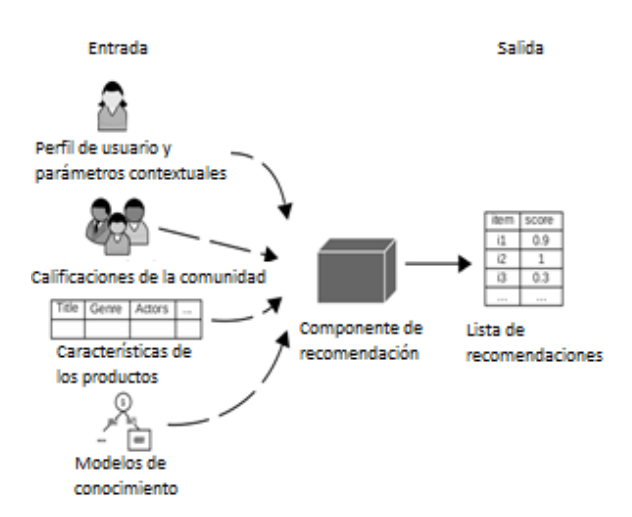
\includegraphics[width=\textwidth]{esquema} \caption{Esquema funcional de un SR. Fuente [\textbf{4}]} \label{fig:etiqueta} \end{figure}

Es decir: sea U el conjunto de usuarios del sistema, sea I el conjunto de ítems en el catálogo. Y sea rec (u, i) la función de utilidad de U → I. R en [0,1]:\\
$RS(u,n) = {i_1, i_2, i_3,...,i_n}$\\
donde $i_1, i_2, i_3,..., i_n \in \textit{I}$ y además\\
%\begin{figure}[h] \centering 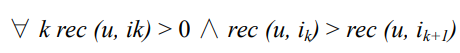
\includegraphics[width=\textwidth]{formula} \caption{}  \end{figure}
$\forall$ k rec (u,$i_k$) $>$ 0 y \textit{rec (u, $i_k$)} $>$ \textit{rec (u, $i_{k+1}$)}\\
\subsection{Filtros}
El mismo autor en [\textbf{4}], de acuerdo al enfoque utilizado para obtener la lista de recomendaciones, clasifica a los SR en:\\
\textbf{1.} \textit{Basados en contenido:} realizan recomendaciones basados en similitudes de los ítems de un catálogo. Dichas recomendaciones pueden realizarse usando calificaciones que han recibido los objetos de forma anónima o bien considerando sus características. Se basan en la premisa de que, si una persona escogió un elemento, entonces le gustarán otros similares. Estos sistemas tienen problemas con los usuarios nuevos, pues requieren saber los intereses del usuario en los objetos del catálogo para poder realizar su trabajo.\\
\textbf{2.} \textit{Basados en conocimiento:} realizan recomendaciones basados en la información que conocen a priori o por medio de la interacción con el usuario. Se basan en la premisa de satisfacer necesidades en vez de intereses. Estos sistemas requieren de una base de conocimientos que defina los criterios que los ítems deben cumplir para poder ser recomendados. En la mayoría de las implementaciones estos sistemas utilizan una estructura taxonómica facetada para multicategorizar los elementos del catálogo. Si ninguno de los ítems coincide con los requerimientos solicitados entonces puede procederse a hacer un relajamiento de alguna restricción o interactuar con el usuario para establecer otro encuadre. Tienen la desventaja de que requieren de un discriminante para ponderar las recomendaciones cuando existe más de un artículo que cumpla con las especificaciones solicitadas. \\
\textbf{3.} \textit{Basados en colaboración:} realizan recomendaciones basados en las calificaciones que los usuarios han hecho sobre los ítems. Estos sistemas trabajan sobre la matriz de calificaciones de los objetos y se basan en la premisa de que debido a que a X le han gustado estos elementos porque los ha calificado de esta manera, entonces le gustarán las cosas que a otros han calificado de forma similar. Estos sistemas tienen problemas con los comportamientos de las calificaciones, pues puede ser que no haya ninguna o bien fueron asignadas al azar; así también con los nuevos elementos en el catálogo puesto que no han recibido ninguna calificación.\\
\textbf{4.} \textit{ Híbridos:} combinan diferentes enfoques para generar las recomendaciones. Pueden ser basados en conocimiento y contenido, para subsanar las debilidades de cada uno de los métodos por separado, o bien basados en colaboración y conocimiento, o inclusive combinar varios métodos para obtener mejores recomendaciones.\\

Sin importar la técnica a seguir, el proceso de obtención de recomendaciones se basa en similaridad. La similaridad es un valor (generalmente de -1 a 1) que indica cuan relacionados están dos componentes. Generalmente se usan las medidas de distancia entre ítems para representar esta medida, por ejemplo: la correlación de Pearson, la distancia cuadrática media, la distancia Manhattan, la distancia del coseno, la distancia del coseno ajustado, etc. Cada una de estas ha sido propuesta por diferentes investigadores como una forma de definir mejores relaciones entre los elementos basados en la información que se posee; aquellos más parecidos serán los que estarán involucrados dentro del cálculo de las recomendaciones. [\textbf{3}] \\
En este trabajo en específico fue utilizado un sistema de recomendación híbrido que combina un SR basado en contenido y uno basado en Colaboración. Ambos emplean la similitud coseno.


\subsection{Ventajas del Enfoque Híbrido}
El sistema híbrido propuesto ofrece varias ventajas en comparación con los enfoques de filtrado colaborativo y basado en contenido por separado:

\begin{itemize}
    \item \textbf{Mejora en la Precisión de las Recomendaciones}: Al combinar ambos enfoques, el sistema puede proporcionar recomendaciones más precisas al aprovechar la información de las interacciones y las características del producto.
    \item \textbf{Mitigación del Problema del Cold Start}: El enfoque híbrido puede manejar mejor el problema del comienzo frío al utilizar características del producto para hacer recomendaciones incluso cuando hay pocos datos de interacción.
    \item \textbf{Personalización Más Efectiva}: La combinación de filtrado colaborativo y basado en contenido permite una personalización más efectiva al integrar las preferencias del usuario y las características del producto.
    \item \textbf{Flexibilidad en Diversos Escenarios}: El enfoque híbrido puede adaptarse a diversos escenarios y tipos de datos, proporcionando recomendaciones relevantes en una variedad de contextos.
\end{itemize}

\section{Estructura del Proyecto}
El sistema está organizado en módulos clave, cada uno responsable de un aspecto específico del proceso de recomendación; pero antes de desglozar la estructura del proyecto, se explicará cómo está conformado el conjunto de datos (\textit{dataset}) que se utilizó.\\

\subsection{Conjunto de datos (\textit{dataset})}

\subsubsection{Fuente\\}
El conjunto de datos fue extraído del sitio web de \textit{kaggle}[\textbf{2}].

\subsubsection{Estructura\\}
El conjunto de datos consta de tres (3) archivos Excel: \textit{customer details} (detalles de los clientes), \textit{product details} (detalles de los productos) e \textit{interactions details} (detalles de las interacciones). Cada fila de cada archivo representa un elemento del conjunto de datos de interés (un cliente en el caso del primer archivo, un producto en el caso del segundo, y, en el caso del tercero, una interacción entre un cliente y un producto).\\
El archivo que contiene los detalles de los clientes, cada columna representa una característica relevante de los clientes (valga la redundancia), por ejemplo: identificador, edad, sexo, producto que compró así como detalles de dicho producto (nombre del artículo, categoría, etc.), tipo de pago, frecuencia con la que compra, temporada de compra, etc.. En en caso del archivo que contiene los detalles de los productos, cada columna representa, de igual modo, una característica a tener en cuenta de cada uno, por ejemplo: identificador único, nombre, categoría, número del modelo, foto, descripción, precio de venta, enlace del producto, etc.. Finalmente, el archivo que contiene las interacciones entre cliente y producto posee en cad columna información relevante sobre cada interacción, como son: identificador del cliente, identificador del producto, tipo de interacción (el cliente 'miró' el producto, indicó que 'le gusta' o lo 'compró'), fecha de la interacción, etc.

\subsection{Filtros (Filters)}
Este módulo implementa las estrategias de recomendación. Se incluyen los siguientes filtros:

\begin{itemize}
    \item \textbf{Filtro Colaborativo (CollaborativeFilter)}: Basado en la similitud de interacciones entre usuarios.
    \item \textbf{Filtro Basado en Contenido (ContentBasedFilter)}: Basado en la similitud de atributos (en este caso, la descripción) entre productos.
\end{itemize}

\subsection{Acceso a los datos (Data Access)}
Módulo responsable de la gestión y recuperación de datos. Incluye los siguientes repositorios:

\begin{itemize}
    \item \textbf{Repositorio Producto (ProductRepository)}: Gestión de datos de productos.
    \item \textbf{Repositorio Cliente (CustomerRepository)}: Gestión de datos de clientes.
    \item \textbf{Repositorio Interacción (InteractionRepository)}: Gestión de interacciones usuario-producto.
\end{itemize}

\subsection{Modelos (Models)}
Define los modelos de datos utilizados en el sistema. Incluye:

\begin{itemize}
    \item \textbf{Contexto (Context)}: Información para aplicar filtros, como el ID del usuario y productos relevantes.
    \item \textbf{Modelo Resultado de Filtro (FilterResultModel)}: Representa los resultados de aplicar un filtro.
    \item \textbf{Modelo Recomendación (RecommendationModel)}: Representa una recomendación individual.
\end{itemize}

\subsection{Services}
Proporciona servicios adicionales que soportan la funcionalidad del sistema, como:

\begin{itemize}
    \item \textbf{Logger}: Registro y seguimiento de actividades del sistema.
\end{itemize}

\section{Métricas}

\section{Conclusión}
El sistema de recomendación híbrido presentado combina las fortalezas del filtrado colaborativo y basado en contenido, ofreciendo un enfoque robusto para la personalización de contenido en plataformas digitales. La integración de estos métodos permite superar las limitaciones individuales y proporcionar recomendaciones más precisas y relevantes, mejorando la experiencia del usuario. La evaluación del sistema demuestra su eficacia en diferentes escenarios y su capacidad para manejar el problema del \textit{comienzo frío} (\textit{cold start}).

\section{Referencias}
\begin{thebibliography}{99}
\bibitem{1}
Google Cloud Team. \textit{How to Build a Recommendation System}. YouTube. \url{https://www.youtube.com/watch?v=F7OTS6qn5Dg&list=PLTjbQZu8nnshv8H5tV0fGh0ECBIXwuHJb}.\\

\bibitem{2}
Pachauri, Shrey. \textit{Sales Ecommerce}. Kaggle. \url{https://www.kaggle.com/datasets/shreypachauri123/sales-ecomerces}.\\

\bibitem{3}
Mendoza Olguín, Gustavo Emilio; Laureano de Jesús, Yadira; Pérez de Celis Herrero, María de la Concepción; \textit{Métricas de similaridad y evaluación para sistemas de recomendación de filtrado colaborativo}, Revista de Investigación en Tecnologías de la Información: RITI, ISSN-e 2387-0893, Vol. 7, N° 14, 2019, ejemplar dedicado a Julio-Diciembre, pages 224-240\\

\bibitem{4}
Dietmar, J.; Zanker, M.; Felfernig, A; Friedrich, G.; \textit{An introduction to recommender systems}, New York: Cambridge, 2011\\

\end{thebibliography}

\end{document}
